\section{335 --- Self Crossing}
You are given an array $ x $ of $ n $ positive numbers. You start at point $ (0,0) $ and moves $ x[0] $ metres to the north, then $ x[1] $ metres to the west, $ x[2] $ metres to the south, $ x[3] $ metres to the east and so on. In other words, after each move your direction changes counter-clockwise.
\par
Write a one-pass algorithm with $ O(1) $ extra space to determine, if your path crosses itself, or not.

 

\paragraph{Example 1:}

\begin{flushleft}
\begin{figure}[H]
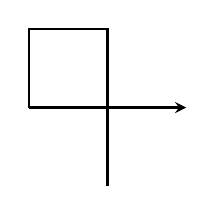
\begin{tikzpicture}
\draw[thick] (0,0) -- ++(0,2) -- ++(-1,0) -- ++(0,-1); 
\draw[thick,>=stealth,->] (-1,1) -- (1,1);
\end{tikzpicture}
\end{figure}
\textbf{Input}: $ [2,1,1,2] $
\\
\textbf{Output}: \texttt{true}
\end{flushleft}

\paragraph{Example 2:}

\begin{flushleft}
\begin{figure}[H]
\begin{tikzpicture}
\draw[thick] (0,0) -- ++(0,1) -- ++(-2,0) -- ++(0,-3) -- ++(4,0);
\draw[thick,>=stealth,->] (-2,-2) -- (2,-2);
\end{tikzpicture}
\end{figure}
\textbf{Input}: [1,2,3,4]
\\
\textbf{Output}: \texttt{false} 
\end{flushleft}

\paragraph{Example 3:}

\begin{flushleft}
\begin{figure}[H]
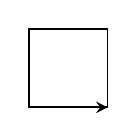
\begin{tikzpicture}
\draw[line width=0.7pt] (0,0) -- ++(0,1) -- ++(-1,0) -- ++(0,-1) -- ++(1,0);
\draw[thick,>=stealth,->] (-1,0) -- (0,0);
\end{tikzpicture}
\end{figure}
\textbf{Input}: $ [1,1,1,1] $
\\
\textbf{Output}: \texttt{true} 
\end{flushleft}

\subsection{Analysis}
实际上相交的情况只有以下三种情况
\begin{enumerate}
\item 第四条边和第一条边相交的情况,需要满足的条件是第一条边大于等于第三条边 ($ x_0\geq x_2 $),第四条边大于等于第二条边 ($ x_3 \geq x_1 $)。同样适用于第五条边和第二条边相交,第六条边和第三条边相交等等,依次向后类推的情况
\begin{figure}[H]
\begin{tikzpicture}
\draw[thick] (0,0) -- ++(0,4) -- ++(-2,0) -- ++(0,-2); 
\draw[thick,>=stealth,->] (-2,2) -- (2,2);
\node (0) at (0.5,3) {{\small $x_0$}};
\node (0) at (-1,4.5) {{\small $x_1$}};
\node (0) at (-2.5,3) {{\small $x_2$}};
\node (0) at (-0.5,2.4) {{\small $x_3$}};
\end{tikzpicture}
\caption{Case 1: $ x_0\geq x_2 $, $ x_3\geq x_1 $}
\end{figure}
\item 第二类是第五条边和第一条边重合相交的情况,需要满足的条件是第二条边和第四条边相等 ($ x_1=x_3 $),第五条边大于等于第三条边和第一条边的差值 ($ x_4\geq x_2 - x_0 $),同样适用于第六条边和第二条边重合相交的情况等等依次向后类推。
\begin{figure}[H]
\begin{tikzpicture}
\draw[thick, color=blue] (0,0) -- ++(0,2) -- ++(-3,0) -- ++(0,-4) -- ++(3,0);
\draw[thick, >=stealth,->, color=red] (0,-2) -- (0,0);
\node at (0.5,1) {{\small $x_0$}};
\node at (-1.5,2.5) {{\small $x_1$}};
\node at (-3.5,0) {{\small $x_2$}};
\node at (-1.5,-2.5) {{\small $x_3$}};
\node at (0.5,-1) {{\small $x_4$}};
\end{tikzpicture}
\caption{Case 2: $ x_1=x_3 $, $ x_4\geq x_2 - x_0 $ }
\end{figure}
\item 第三类是第六条边和第一条边相交的情况,需要满足的条件是第四条边大于等于第二条边($ x_3 \geq x_1 $),第三条边大于等于第五条边 ($ x_2 \geq x_4 $),第五条边大于等于第三条边和第一条边的差值 ($ x4 \geq x_2 - x_0 $),第六条边大于等于第四条边和第二条边的差值 ($ x_5\geq x_3-x_1 $),同样适用于第七条边和第二条边相交的情况等等依次向后类推。
\begin{figure}[H]
\begin{tikzpicture}
\draw[thick, color=blue] (0,0) -- ++(0,3) -- ++(-3,0) -- ++(0,-5) -- ++(5,0) -- ++(0,3);
\draw[thick, >=stealth,->, color=red] (2,1) -- (-1,1);
\node at (0.5,2.3) {{\small $x_0$}};
\node at (-1.5,3.5) {{\small $x_1$}};
\node at (-3.5,0.5) {{\small $x_2$}};
\node at (-0.5,-2.5) {{\small $x_3$}};
\node at (2.5,-0.5) {{\small $x_4$}};
\node at (1,0.5) {{\small $x_5$}};
\end{tikzpicture}
\caption{Case 3: $ x_3\geq x_1 $, $ x_2\geq x_4 $, $ x_4\geq x_2 - x_0 $, $x_5\geq x_3-x_1$}
\end{figure}
\end{enumerate}
\setcounter{algorithm}{0}
\begin{algorithm}[H]
\caption{Three Cases}
\begin{algorithmic}[1]
\Procedure{IsSelfCrossing}{$x, L$}
\For{$i:=3$ \textbf{to} $L-1$}
\State $\ast$ Case 1
\State $x_0 = x[i-3]$, $ x_1= x[i-2] $, $ x_2 = x[i-1] $, $ x_3 = x[i] $
\If{$ x_0 \geq x_2 $ \textbf{and} $ x_3\geq x_1 $}
\State \Return \texttt{true}
\EndIf
\If{$i\geq 4$}
\State $\ast$ Case 2
\State $x_0 = x[i-4]$, $ x_1= x[i-3] $, $ x_2 = x[i-2] $, $ x_3 = x[i-1] $, $ x_4 = x[i] $
\If{$x_1=x_3$ \textbf{and} $ x_4\geq x_2-x_0 $}
\State \Return \texttt{true}
\EndIf
\EndIf
\If{$i\geq 5$}
\State $\ast$ Case 3
\State $x_0 = x[i-5]$, $ x_1= x[i-4] $, $ x_2 = x[i-3] $, $ x_3 = x[i-2] $, $ x_4 = x[i-1] $, $ x_5 = x[i] $
\If{$x_3\geq x_1$ \textbf{and} $ x_2\geq x_4 $ \textbf{and} $ x_4\geq x_2-x_0 $ \textbf{and} $ x_5\geq x_3 -x_1 $}
\State \Return \texttt{true}
\EndIf
\algstore{335algo}
\end{algorithmic}
\end{algorithm}
\begin{algorithm}[H]
\begin{algorithmic}[1]
\algrestore{335algo}
\EndIf
\EndFor
\EndProcedure
\end{algorithmic}
\end{algorithm}
\setcounter{lstlisting}{0}
\begin{lstlisting}[style=customc, caption={Three Cases}]
bool isSelfCrossing( vector<int>& x )
{
    int y[6] = {0};

    for( size_t i = 3; i < x.size(); ++i )
    {
        y[0] = x[i - 3];
        y[1] = x[i - 2];
        y[2] = x[i - 1];
        y[3] = x[i];

        //case 1:
        if( ( y[0] >= y[2] ) && ( y[3] >= y[1] ) )
        {
            return true;
        }

        //case 2:
        if( i >= 4 )
        {
            y[0] = x[i - 4];
            y[1] = x[i - 3];
            y[2] = x[i - 2];
            y[3] = x[i - 1];
            y[4] = x[i];

            if( ( y[3] == y[1] ) && ( y[4] >= y[2] - y[0] ) )
            {
                return true;
            }

        }

        //case 3:
        if( i >= 5 )
        {
            y[0] = x[i - 5];
            y[1] = x[i - 4];
            y[2] = x[i - 3];
            y[3] = x[i - 2];
            y[4] = x[i - 1];
            y[5] = x[i];

            if( ( y[3] >= y[1] ) && ( y[2] >= y[4] ) && ( y[4] >= y[2] - y[0] ) && ( y[5] >= y[3] - y[1] ) )
            {
                return true;
            }
        }

    }

    return false;
}

\end{lstlisting}